\section{Visualization of Network and Tree Data}

TODO: talk about connection and containment marks as in Munzner's book before referring to them. Basically, node-link diagrams use connection and space-filling uses containment.

\subsection{Node-Link Diagrams}
The most common visual encoding for network and tree data is with node-link diagrams, where nodes are represented as points and links connecting them are drawn as curves. Node-link diagrams use links to indicate relationships between nodes. We further discuss layouts using this visual encoding for network data with different constraints: rooted tree, directed graph and general graph.

\subsubsection{Tree Layout}
A classic algorithm by Reingold and Tilford~\cite{Reingold1981} produces a tidy tree layout satisfying the following aesthetic rules:
\begin{enumerate}
	\item Nodes at the same level of the tree should lie along a straight line, and the straight lines defining the levels should be parallel.
	\item A left son should be positioned to the left of its father and a right son to the right.
	\item A father should be centered over its sons.
\end{enumerate} 

However, the layout is space-inefficient, leaving void space at the root side of the tree (\autoref{fig:lr-tree-tidy}). Marriott and Sbarski~\cite{Marriott2007} relax the rule that a parent must be placed at the center of its children, slightly shifting branches or nodes to produce a narrower tree. In practice, nodes have their sizes rather than single points, and their heights can be different. Van der Ploeg~\cite{VanderPloeg2014} relaxes the layering requirement to produce a shorter tree (\autoref{fig:lr-tree-tidy-non-layer}).

%\begin{figure}[!htb]
%	\centering
%	\includegraphics[width=.5\columnwidth]{tree-flare}
%	\caption{The data--frame model. \emph{Source:~\cite{Klein2003}}.}
%	\label{fig:data-frame-model}
%\end{figure}
\begin{figure}[!htb]
\centering
\subcaptionbox{Standard Reingold--Tilford algorithm. \is{Nguyen2002}\label{fig:lr-tree-tidy}}{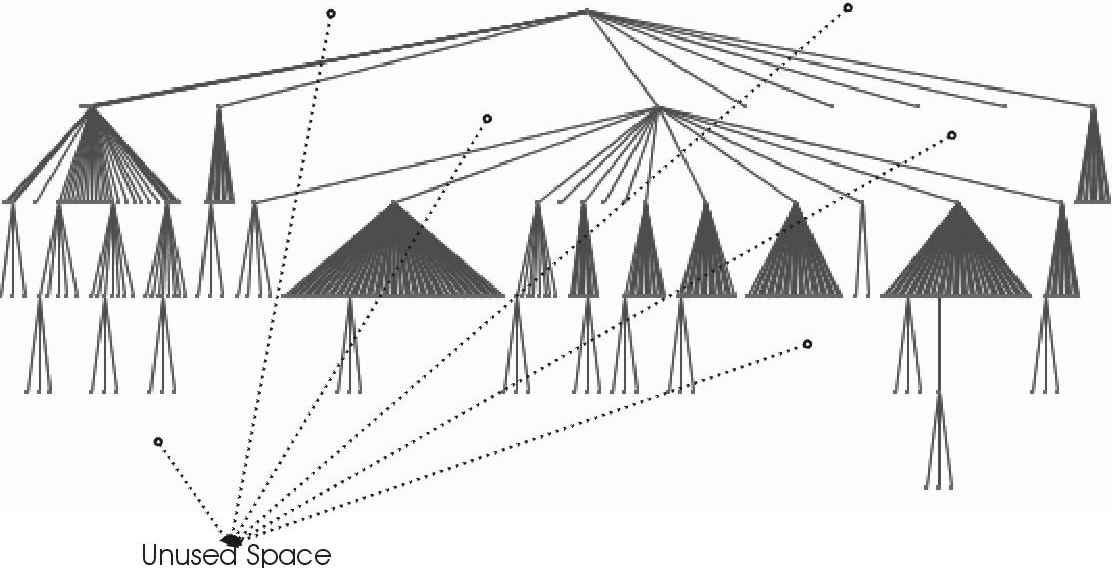
\includegraphics[height=.315\columnwidth]{tree-tidy}}
\hfill
\subcaptionbox{Relaxed layering for shorter layout. \is{VanderPloeg2014}\label{fig:lr-tree-tidy-non-layer}}{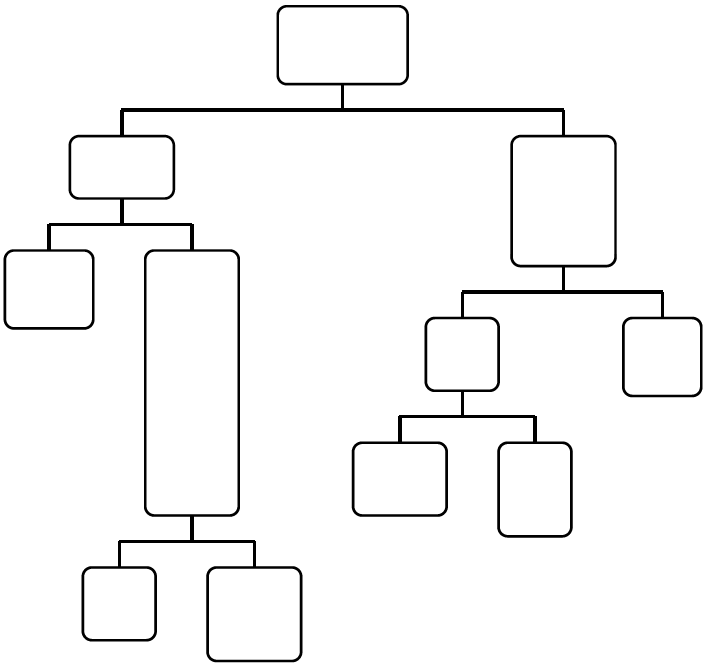
\includegraphics[height=.315\columnwidth]{tree-tidy-non-layer}}
\caption{Tree layouts.}
\end{figure}

Conventionally, tree layouts are rectilinear, children growing from the parent node from left to right or top to bottom. However, they can also be arranged radially: children are located along a circular arc of their parent. The depth of the tree is encoded as distance away from the center of the circle. Reingold--Tilford algorithm can be modified to show a radial tree as in \autoref{fig:lr-tree-radial}. Using the same dataset, \autoref{fig:lr-tree-rect} shows a conventional tree from left to right.

\begin{figure}[!htb]
\centering
\subcaptionbox{Conventional tree from left to right. \label{fig:lr-tree-rect}}{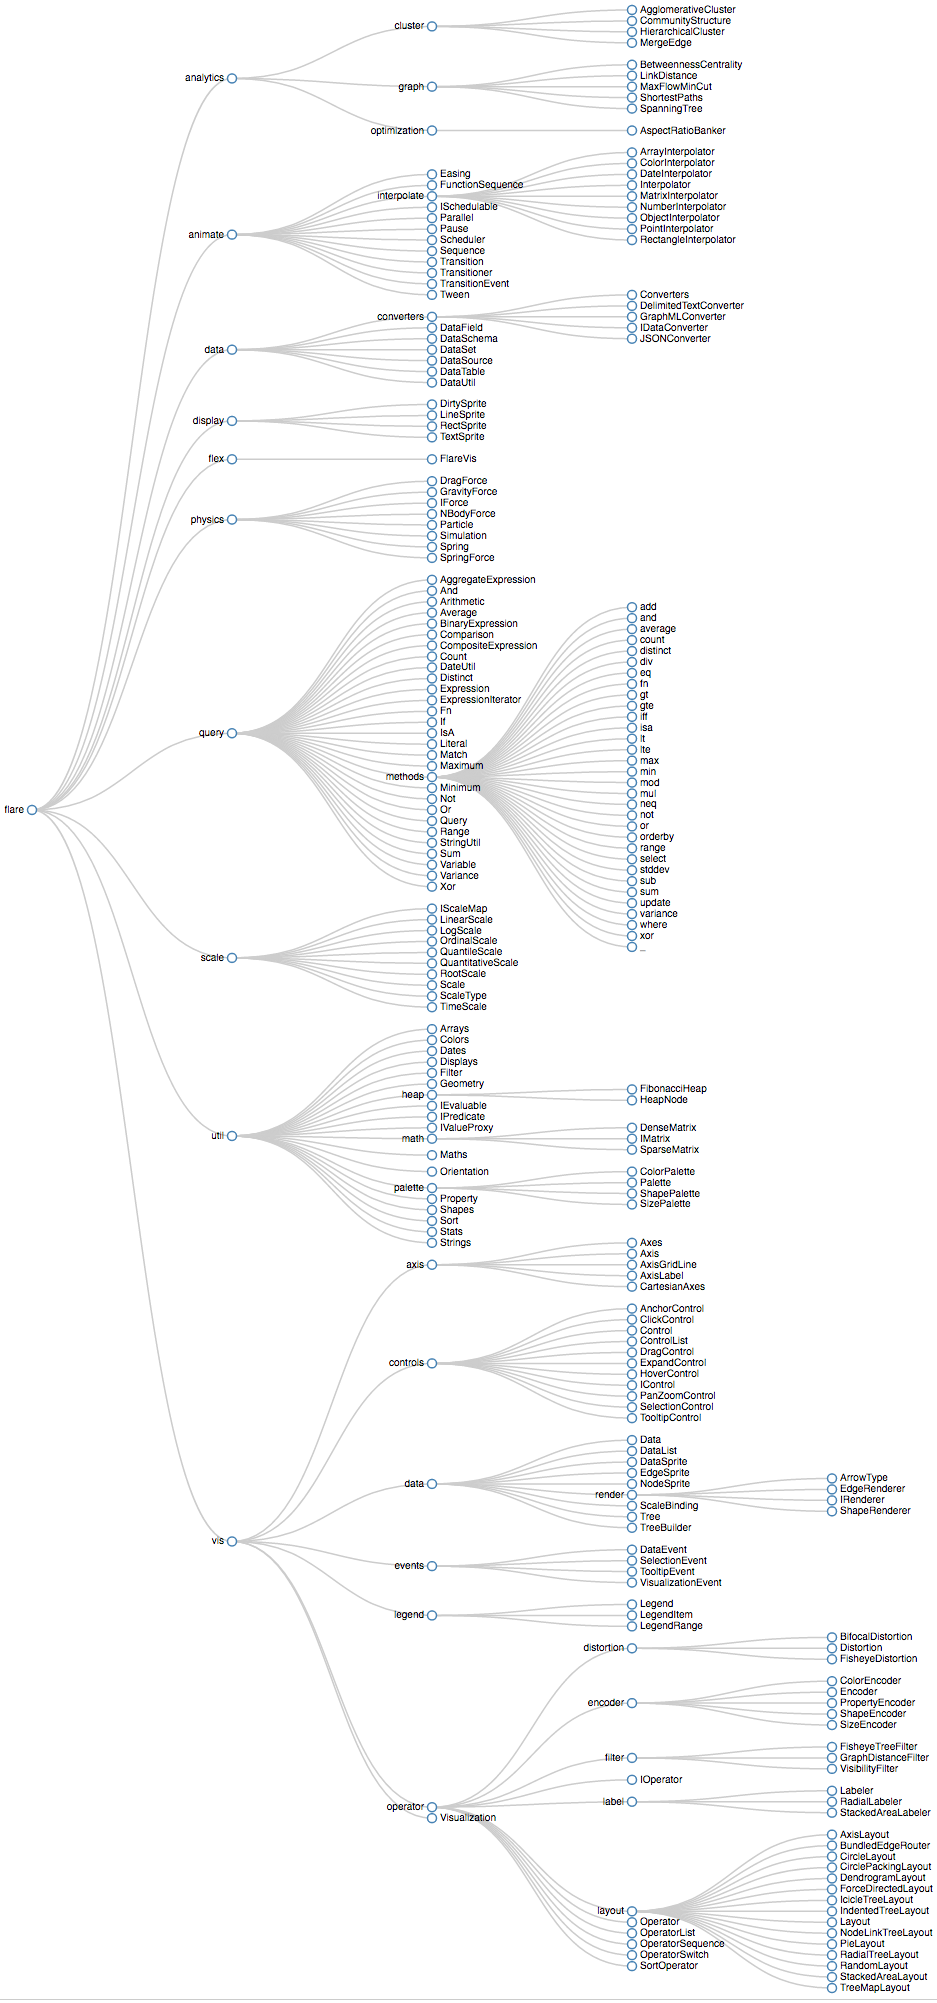
\includegraphics[height=.69\columnwidth]{tree-rect}}
\hfill
\subcaptionbox{Radial tree. Depth is encoded as distance away from the center. \label{fig:lr-tree-radial}}{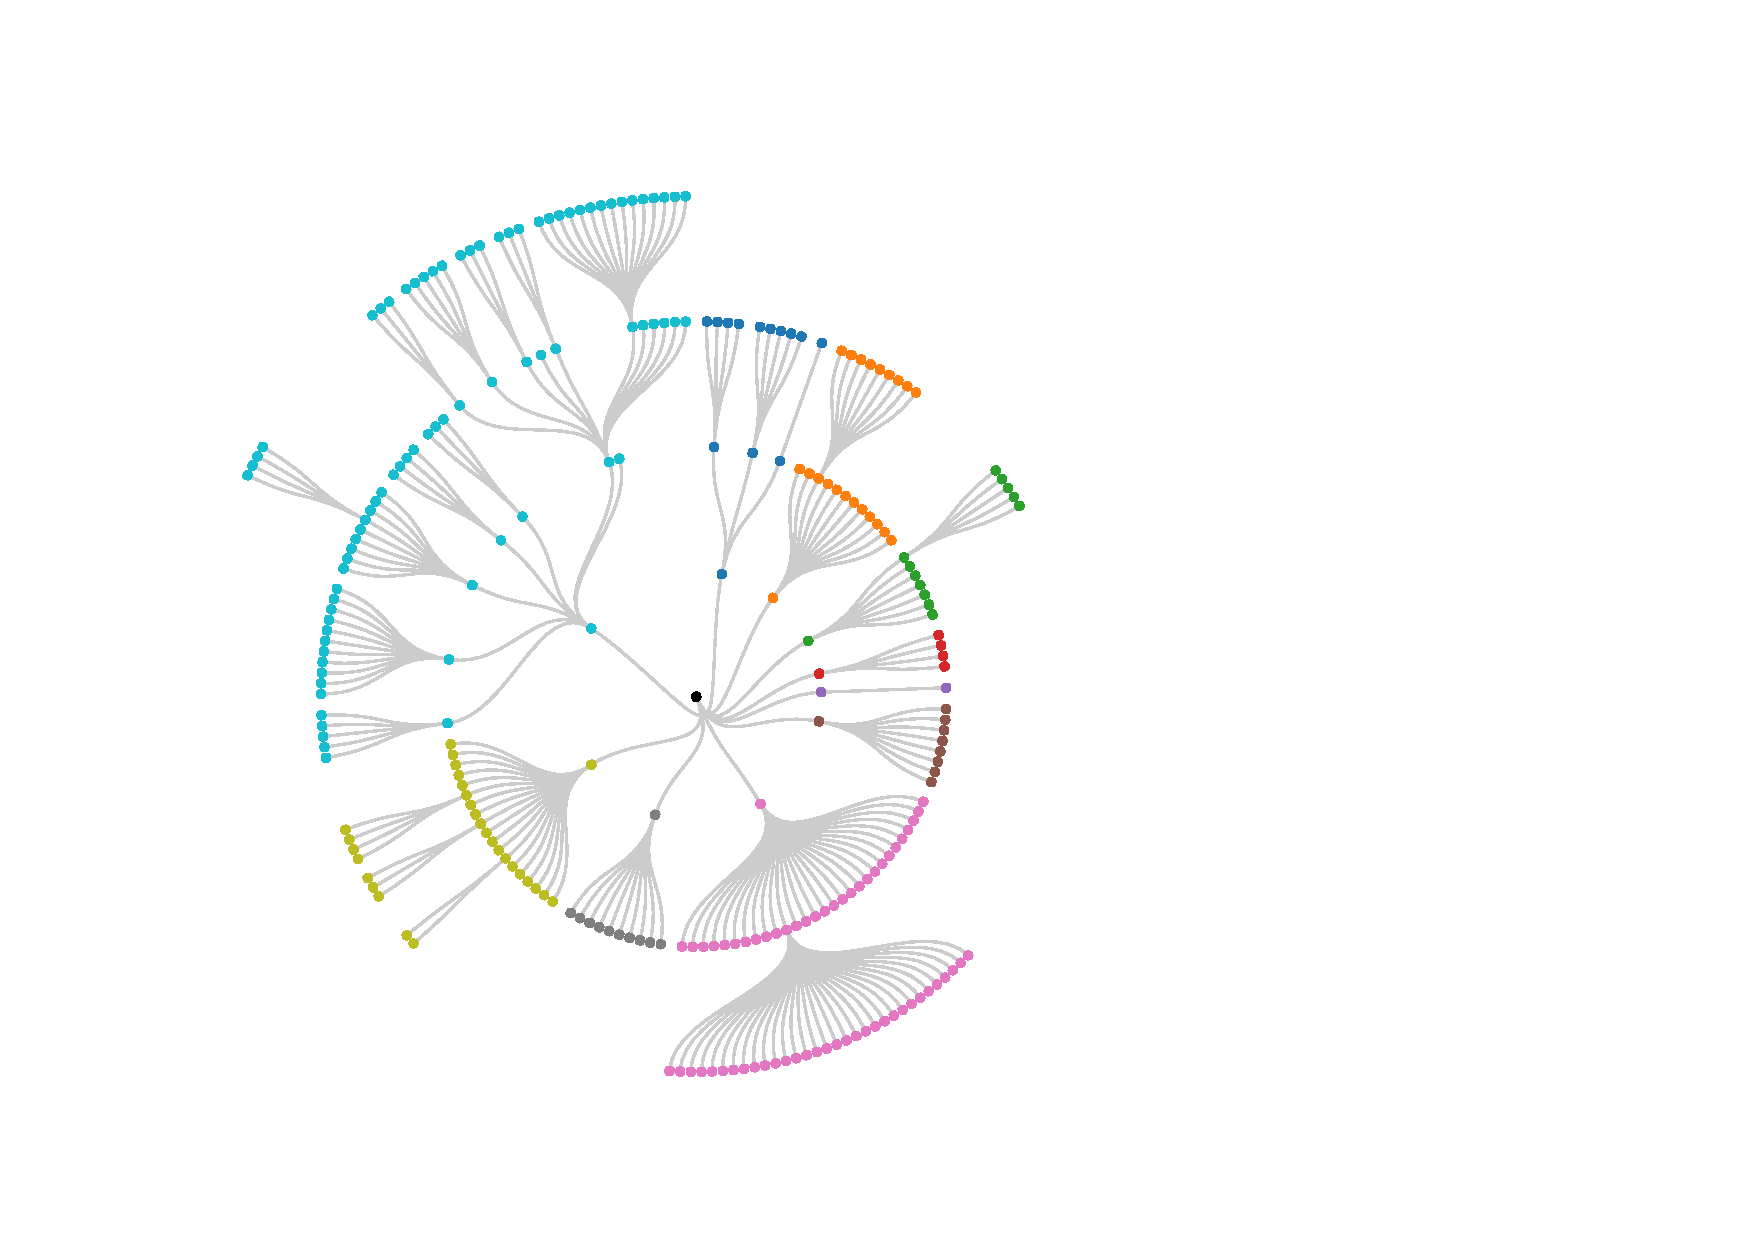
\includegraphics[height=.69\columnwidth]{tree-radial}}
\caption{Tree layouts with different orientations. TODO: regenerate -- remove text, reduce node size 1-2px to avoid overlap, make links darker}
\end{figure}
  
\subsubsection{Hierarchical Graph Layout}	
The most popular method of drawing directed graphs is the Sugiyama framework~\cite{Sugiyama1981}, separating the nodes into layers to show the hierarchy effectively. \autoref{fig:lr-layered-graph} shows an example of layered graphs. The framework consists of four steps.

\begin{figure}[!htb]
	\centering
	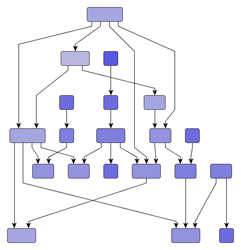
\includegraphics{layered-graph}
	\caption{A layered graph. \textrm{\emph{Image source: documentation of yWorks.}}}
	\label{fig:lr-layered-graph}
\end{figure}

\begin{enumerate}
	\item \emph{Cycle removal}. If the input graph contains directed cycles, temporarily reverse the direction of some edges to make the it acyclic.
	\item \emph{Layer assignment}. Nodes are assigned to horizontal layers which determines their y-coordinate.
	\item \emph{Vertex ordering}. Within each layer, the nodes are ordered to minimize edge crossings between adjacent layers.
	\item \emph{Horizontal coordinate assignment}. The x-coordinate of each node is determined, typically aiming to make edges straight.
\end{enumerate}

\subsubsection{Force-Directed Layout}
Force-directed layout is a popular method to visualize general graphs using node-link metaphor~\cite{Eades1984}. It positions nodes based on a simulation of physical forces: spring-like attractive forces attract nodes, and repulsive forces like those of electrically charged particles push them away from each other. The layout usually starts with a random arrangement of nodes and then iteratively refines their locations according to the behaviors of these simulated forces. The layout stops when the simulation reaches a stable state or a maximum number of iterations. \autoref{fig:lr-force-directed-idea} illustrates the idea of physical simulation, and \autoref{fig:lr-force-directed-example} shows an example of a layout with color indicating node type.

\begin{figure}[!htb]
\centering
\subcaptionbox{A physical simulation. \label{fig:lr-force-directed-idea}}{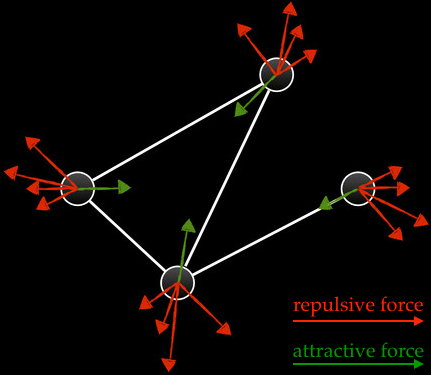
\includegraphics[height=.3\columnwidth]{force-directed-idea}}
\hfill
\subcaptionbox{An example with color showing node type. \label{fig:lr-force-directed-example}}{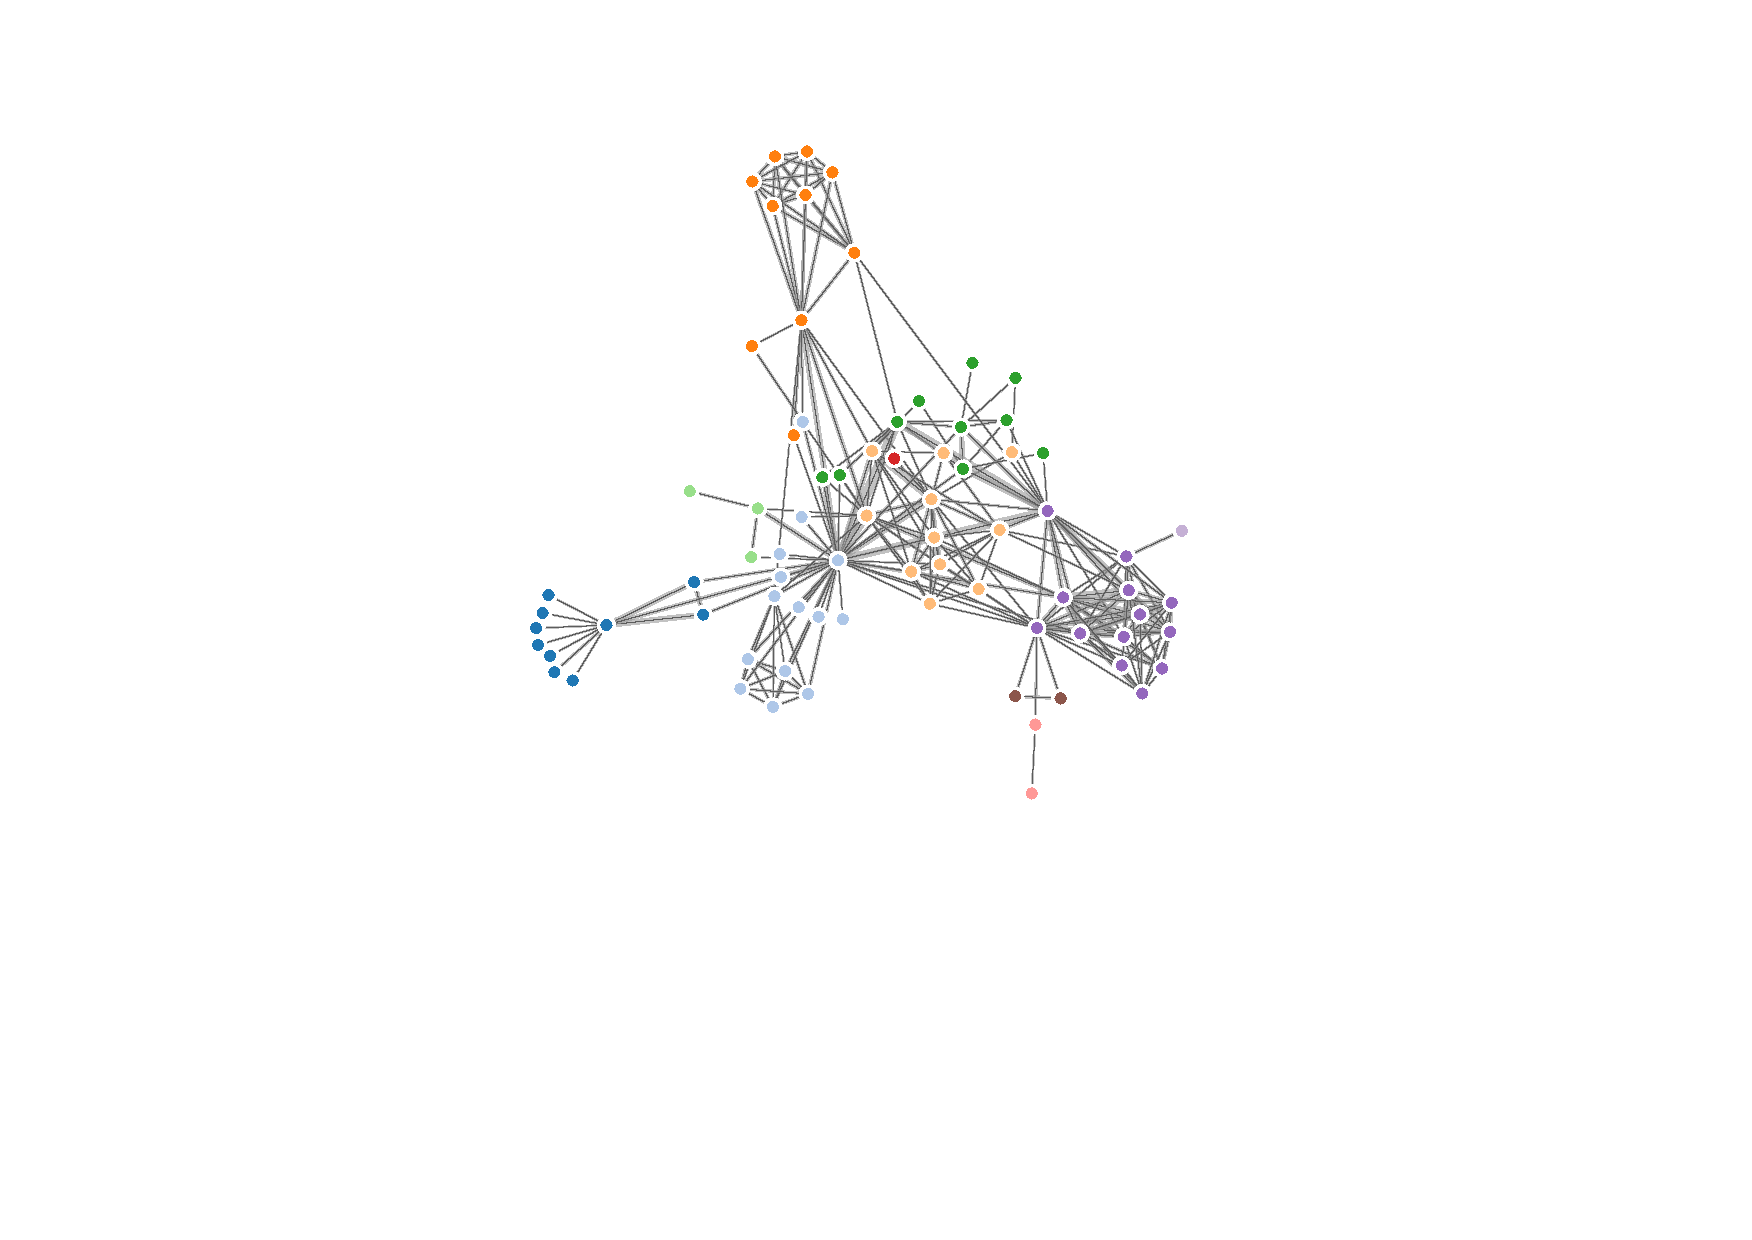
\includegraphics[height=.6\columnwidth]{force-directed-example}}
\caption{Force-directed layout.}
\end{figure}

Force-directed layout is aesthetically pleasing, aiming to produce uniform edge length, symmetry and even node distribution~\cite{Fruchterman1991}. However, a major weakness of this layout is scalability, both in terms of the visual complexity and running time~\cite{Munzner2014}. The layout quickly degenerates into a hairball of visual clutter with even a few hundred nodes. Another limitation is its nondeterministic output: the layout looks different each time it runs, breaking user mental model.

\subsection{Matrix Views}
A network can be represented by an adjacency matrix. Each row and column of the matrix corresponds to a node, and a cell indicates whether the pair of corresponding nodes is connected in the network. Additional information about edges are often encoded to the visual representation of cells using color, shape and size. Matrix views can also show weighted networks, where each link has an associated quantitative value attribute, by encoding with an ordered visual channel such as luminance or size. \autoref{fig:lr-matrix} shows examples of matrix views, compared with node-link diagrams of the same dataset.

\begin{figure}[!htb]
\centering
\subcaptionbox{Comparison with a small network. \label{fig:lr-matrix-1}}{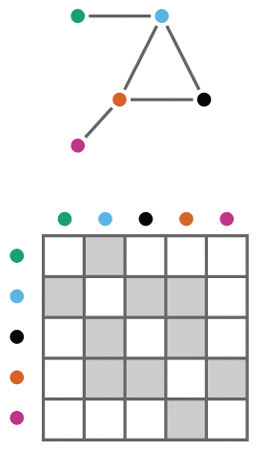
\includegraphics[height=.39\columnwidth]{matrix-1}}
\hfill
\subcaptionbox{Matrix view of larger network. \label{fig:lr-matrix-2}}{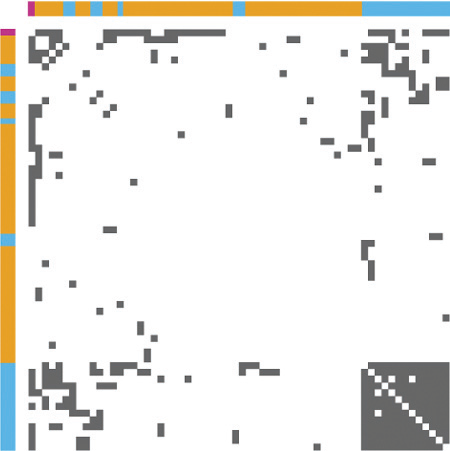
\includegraphics[height=.39\columnwidth]{matrix-2}}
\hfill
\subcaptionbox{Force-directed layout of larger network. \label{fig:lr-matrix-3}}{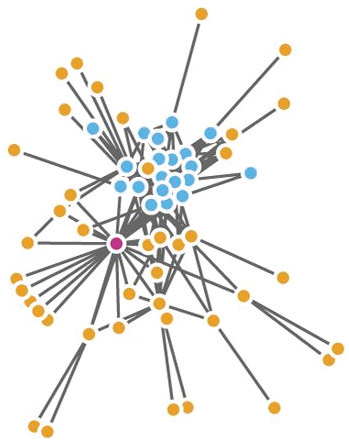
\includegraphics[height=.39\columnwidth]{matrix-3}}
\caption{Comparison of node-link diagrams and matrix views. Gray cells indicate edge connectivity. \is{Munzner2014}}
\label{fig:lr-matrix}
\end{figure}

A major strength of matrix views is the scalability. It can easily show a networks with thousands of nodes and millions of edges without suffering from the cluttering issue as in node-link diagrams. Matrix views are stable, adding a new node or edge will only cause a small visual change. Whereas, adding a new item in a force-directed view may lead to a major change~\cite{Munzner2014}. Nodes, as columns and rows in a matrix view, can be reordered, allowing to reveal outliers, clusters, and patterns of the network~\cite{Henry2007}.

A major weakness of matrix views is their difficulty in exploring the topological structure of the network, such as path tracing and searching local topological neighborhoods a small number of hops from a target node. This because they show links in a more indirect way than the direct connections of node-link diagrams -- a trade-off for their strength in avoiding clutter. Another weakness of matrix views is unfamiliarity: users easily interpret small node-link diagrams but requires training to understand matrix views~\cite{Munzner2014}. A study shows that for many low-level abstract network tasks, node-link diagrams are best for small networks and matrix views are best for large networks~\cite{Ghoniem2005}.

\subsection{Space-Filling Techniques}
Space-filling techniques only apply to tree data and uses \emph{containment} to represent hierarchical relationships, placing child nodes within their parent node. Treemap~\cite{Shneiderman1992} represents a node as a rectangle, which is recursively subdivided into smaller rectangles, each represents a child of the node. The rectangle size is proportional to an attribute of the node. The original motivation of treemap is to analyze the utilization of storage space on a hard disk. Each leaf node represents a computer file, and the node size encodes the file size. The size of a parent node simply maps to the folder size. Color is also commonly used to encode additional information to nodes such as file type. \autoref{fig:lr-treemap} shows such an example of treemap.

\begin{figure}[!htb]
	\centering
	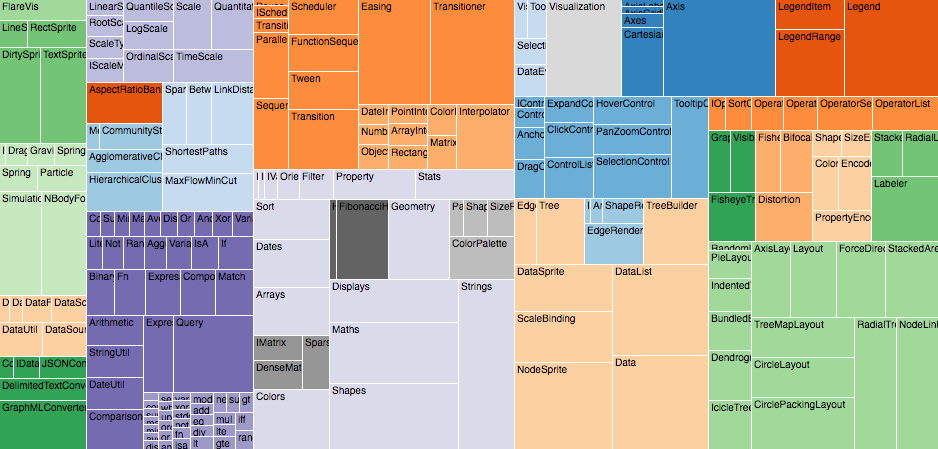
\includegraphics[width=\columnwidth]{treemap}
	\caption{Treemap.}
	\label{fig:lr-treemap}
\end{figure}

Treemap is very effective when size is the most important feature to be displayed. It easily spots outliers of very large attribute values such as large files. However, containment is not as effective as connection in node-link diagrams for tasked focused on topological structure. It is difficult to identify the path of a given node, thus suitable for hierarchies with few a few levels. To improve understanding of the tree structure, borders of nodes can be added or using shading~\cite{Wijk1999}.

Alternatively, other space-filling techniques have been proposed to better represent the hierarchical structure. \autoref{fig:lr-other-space-filling} shows the three techniques that we discuss next using the same dataset as in \autoref{fig:lr-treemap} for treemap. 

Circle packing~\cite{Wang2006} also employs containment to represent hierarchy, but using circles to represent nodes. Circle sizes correspond to some node values. All child nodes are packed into their parent node so that they are tangent to some of their sibling nodes. This method is less space-efficient than treemap but provides better hierarchy structure.

Icicle plot~\cite{Kruskal1983} does not strictly use containment; it places child nodes under their parent node. Similar to treemap, icicle plot uses rectangles to represent nodes, but they all share the same height. Therefore, node width corresponds to some attribute value. Icicle plot shows parent nodes explicitly, making it more effective in tasks related to them such as comparing directories by size. The direct trade-off is space for showing those parent nodes. Icicle plot shows the tree structure and supports path tracing more effectively than treemap. However, small leaf nodes are very thin and difficult to read its label or interact with.

Sunburst~\cite{Zhang2000} is a radial version of icicle plot. It places child nodes under their parent node in a circular layout. Root node is at the center and deeper levels are further away from it. The angle swept out by a node, or a curved segment, corresponds to its value. Color is also commonly used to represent additional information.

\begin{figure}[!htb]
\centering
\subcaptionbox{Icicle plot. \label{fig:lr-icile}}{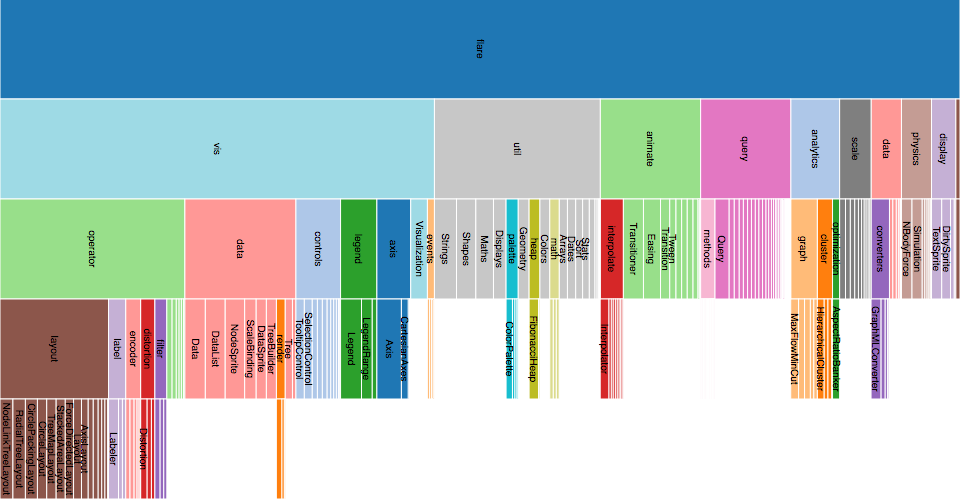
\includegraphics[width=\columnwidth]{icicle-plot}}

\vspace{.5\baselineskip}

\subcaptionbox{Circle packing. \label{fig:lr-circle-pack}}{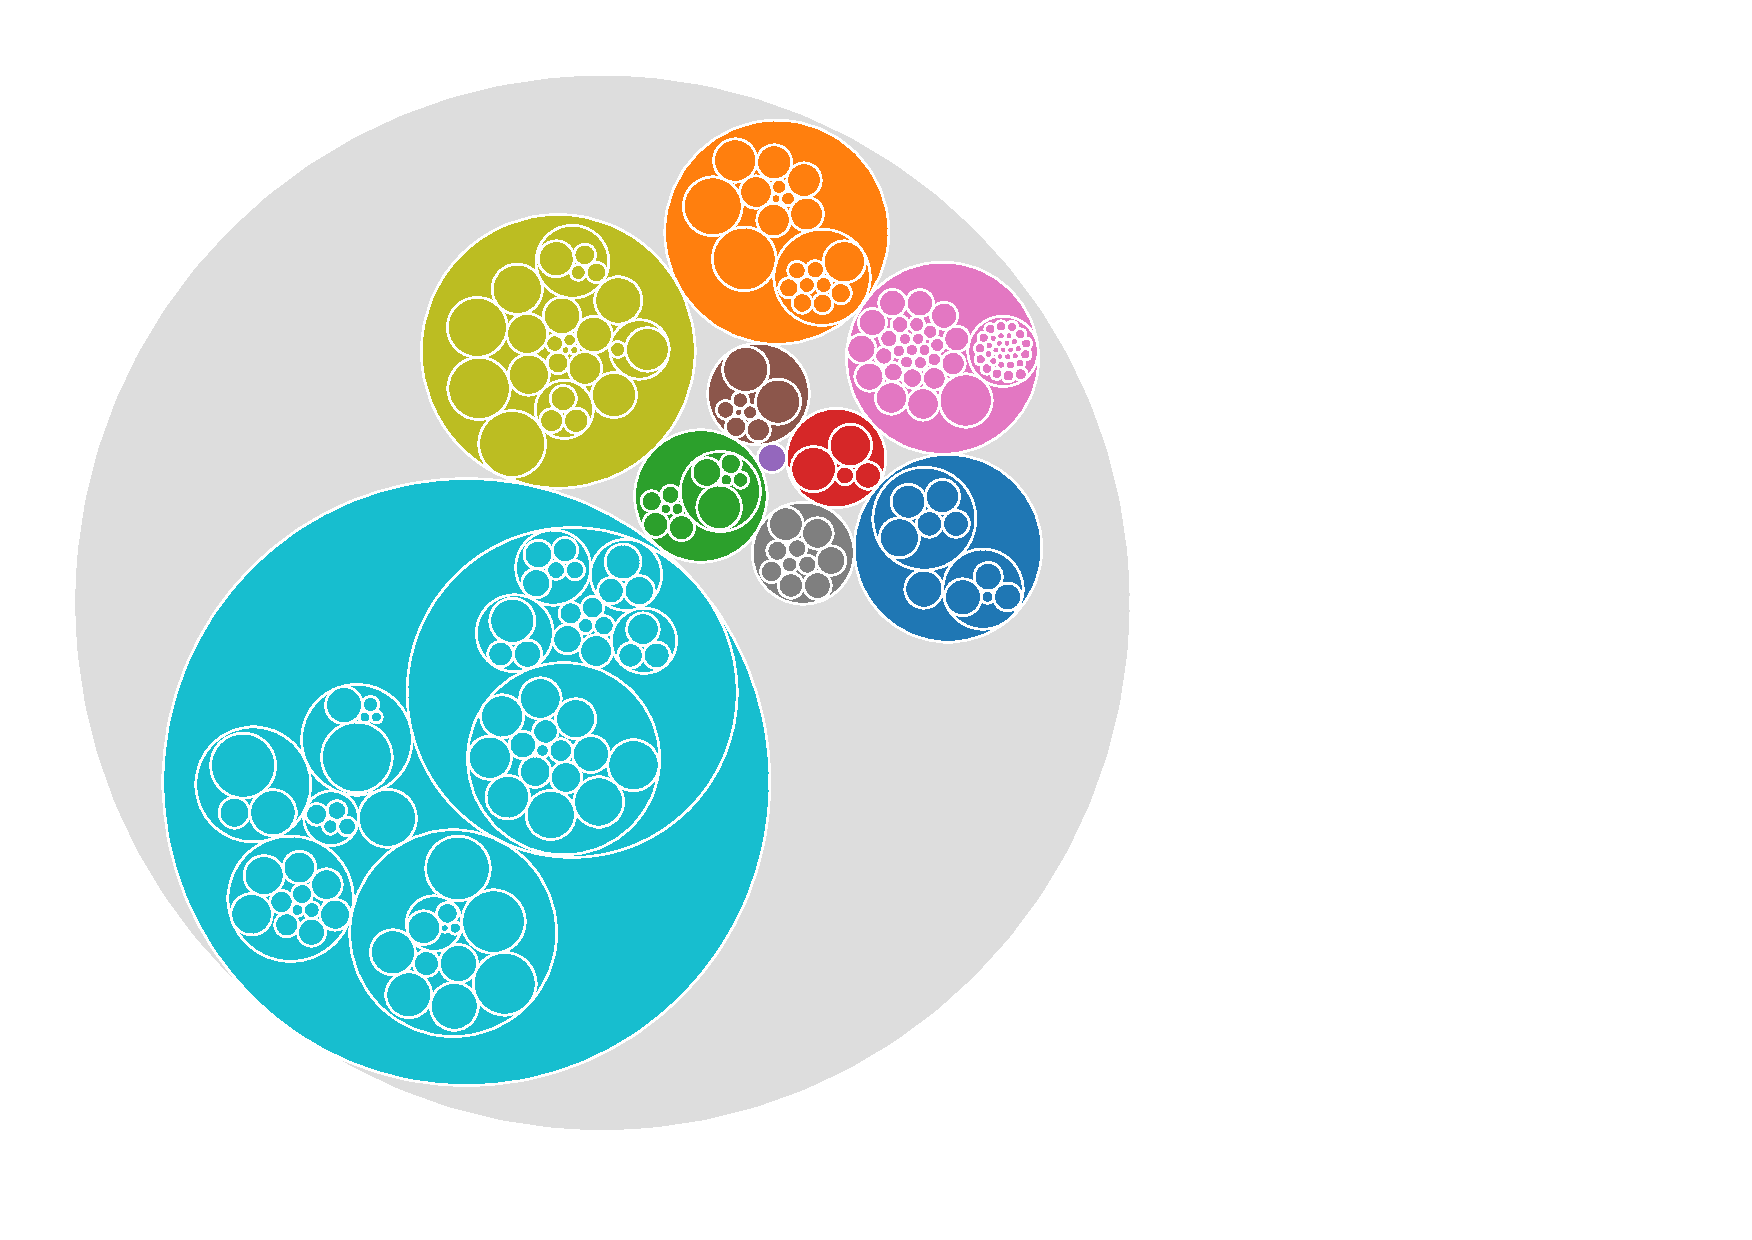
\includegraphics[width=.48\columnwidth]{circle-pack}}
\hfill
\subcaptionbox{Sunburst. \label{fig:lr-sunburst}}{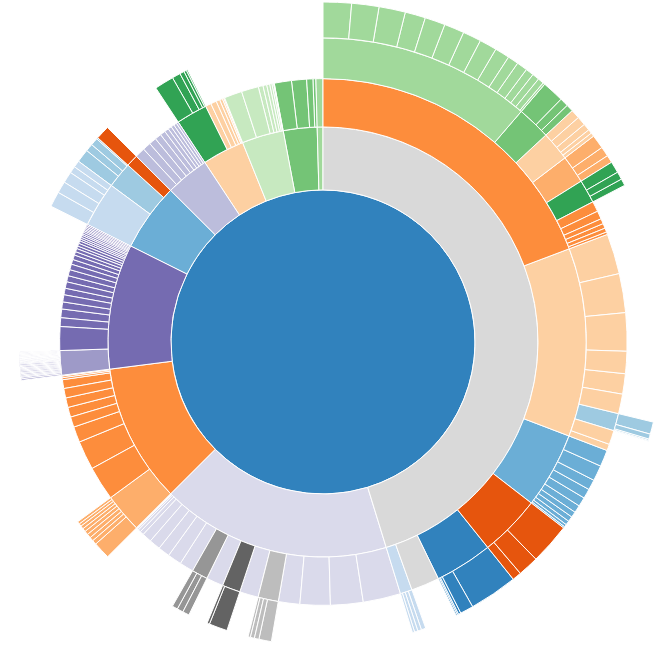
\includegraphics[width=.48\columnwidth]{sunburst}}
\caption{Other space-filling techniques. All sub-figures use the same dataset as in \autoref{fig:lr-treemap}.}
\label{fig:lr-other-space-filling}
\end{figure}


%circle packing: https://bl.ocks.org/mbostock/4063530
%sunburst: http://bl.ocks.org/mbostock/4348373
%treemap: https://bl.ocks.org/mbostock/4063582
%icile: https://bl.ocks.org/mbostock/1005873